
	\subsection{Méthodes d'optimisation orientées source}
	
	Une approche classique consiste à minimiser l'écart entre les mesures des capteurs et les concentrations simulées par un modèle de dispersion. Pour cela, une des techniques les plus courantes consiste à définir une fonction-coût $\CostF$ pour représenter cet écart, puis calculer un estimateur des moindres carrés pour chercher à le minimiser. En reprenant la notation fournie par l'équation \eqref{eq_relation_SR_non_parametrique}, on a alors:
	
	\begin{equation}
	\label{eq_moindres_carres}
	\CostF(\VecSigma) = || \VecObs - \MatH\VecSigma||_2^2
	\end{equation}
	où $||\cdot||_2$ désigne la norme $L_2$.\\
	
	Dans \cite{Kathirgamanathan2002}, un point source instantané est estimé, caractérisé par sa masse totale émise, sa position et son instant d'émission. L'étude qui y est menée met notamment l'accent sur l'influence du dimensionnement du réseau de capteurs sur la performance de la reconstruction : au moins trois points de mesure sont nécessaires, et la distance entre les différents capteurs influe sur la qualité de l'estimation.\\
	
	Dans \cite{Ryall2001}, ce sont des zones d'émission plus grandes qui sont estimées pour des rejets de gaz à effet de serre sur plusieurs années. \\
	
	Dans \cite{Matthes2005}, une approche en deux temps est formulée afin de résoudre un problème de complexité proportionnellement croissante au nombre de capteurs. Dans une première étape, les mesures individuelles de chaque capteur produisent des ensembles de positions probables pour la source. Dans un deuxième temps, ces ensembles sont comparés pour estimer la meilleure position en faisant varier l'intensité de la source à retrouver. \\
	
	Dans certaines situations, la résolution de \eqref{eq_moindres_carres} nécessite une contrainte supplémentaire. C'est par exemple le cas dans \cite{Martinez2013}, où le profil des rejets de xénon sous forme de brèves émissions (\textit{short bursts}) en faible nombre est pris en compte. Concrètement, ce phénomène est illustré par un grand nombre de zéros dans les observations. On parle alors de \textit{sparsité}. Pour compenser ce problème, un terme régularisant suivant une norme $L_1$ est ajouté à la fonction-coût et donne de meilleurs résultats:
	
	\begin{equation}
	\label{eq_regularisation_L1}
	\CostF(\VecSigma) = || \VecObs - \MatH\VecSigma||_2^2 + \alpha||\VecSigma||_1
	\end{equation}
	
	Le facteur $\alpha$ permet de quantifier l'importance que doit avoir le terme régularisant par rapport au premier terme quadratique. Dans d'autres cas, une utilisation de la norme $L_1$ sur l'ensemble de la fonction-coût est préférée, et $\CostF$ prend alors la forme suivante:
	
	\begin{equation}
	\label{eq_moindres_VA}
	\CostF(\VecSigma) = || \VecObs - \MatH\VecSigma||_1
	\end{equation}
	
	
	C'est le cas dans \cite{Cheng2008}, où l'argument de la sparsité est de nouveau mis en avant. En effet, dans cette étude, le domaine des solutions à explorer est relativement important, et le nombre de points pouvant potentiellement représenter une source reste faible par rapport au nombre total de points explorables. Le principe de la minimisation $L_1$ est également repris dans \cite{Konda2010}, où un modèle de dispersion à bouffées est utilisé pour simuler les observations et effectuer les calculs de concentrations aux points sources candidats. \\
	
	Même si cette approche permet globalement d'obtenir de bons résultats, le nombre de calculs de dispersion peut se révéler important, voire excessif selon le domaine considéré. En effet, pour chaque source potentielle, il faut lancer une instance du modèle pour simuler les concentrations qu'auraient mesurées les capteurs : on parle d'\text{approche orientée source}. Une façon de résoudre à ce problème est expliquée dans le paragraphe suivant.\\
	
	
	\subsection{Méthodes d'optimisation orientées récepteur}
	
	 L'approche par optimisation peut être utilisée en conjonction avec un modèle de dispersion dit \textit{adjoint}, ce qui revient à transformer le champ d'émission de \eqref{eq_relation_SR_non_parametrique} en un champ de rétro-émissions issues des capteurs, comme illustré sur les figures \ref{schema_probleme_direct} et \ref{schema_probleme_inverse}.
	 Pour cela, il faut définir le problème dual à celui posé par l'équation d'advection-diffusion \eqref{eqn_advection_diffusion} en inversant la flèche du temps et le sens du vent.  Par le principe de symétrie présenté dans \cite{Hourdin2006a}, on peut alors introduire la notion de \textit{rétro-transport} ou \textit{backtracking} en  réécrivant l'équation d'advection-diffusion sous la forme : 
	 
	 \begin{equation}
	 \label{eqn_advection_diffusion_backward}
	 \dfrac{-\partial C^*}{\partial t} - \nabla \cdot(C^*\bm{\vec{u}}) = \nabla \cdot (\bm{K}\nabla C^*) + \VecObs
	 \end{equation}
	 
	 où $C^*$ est un champ de concentrations conjuguées, ou \textit{rétro-concentrations}, dont les valeurs sont obtenues par des rétro-rejets virtuels depuis les capteurs vers la source. Cette méthodologie est dite \textit{orientée récepteurs}, et permet un certain gain en temps de calcul si le nombre de sources potentielles est supérieur au nombe de capteurs présents dans le domaine. \\
	 
	\begin{figure}[h]
		\begin{subfigure}{0.5\textwidth}
			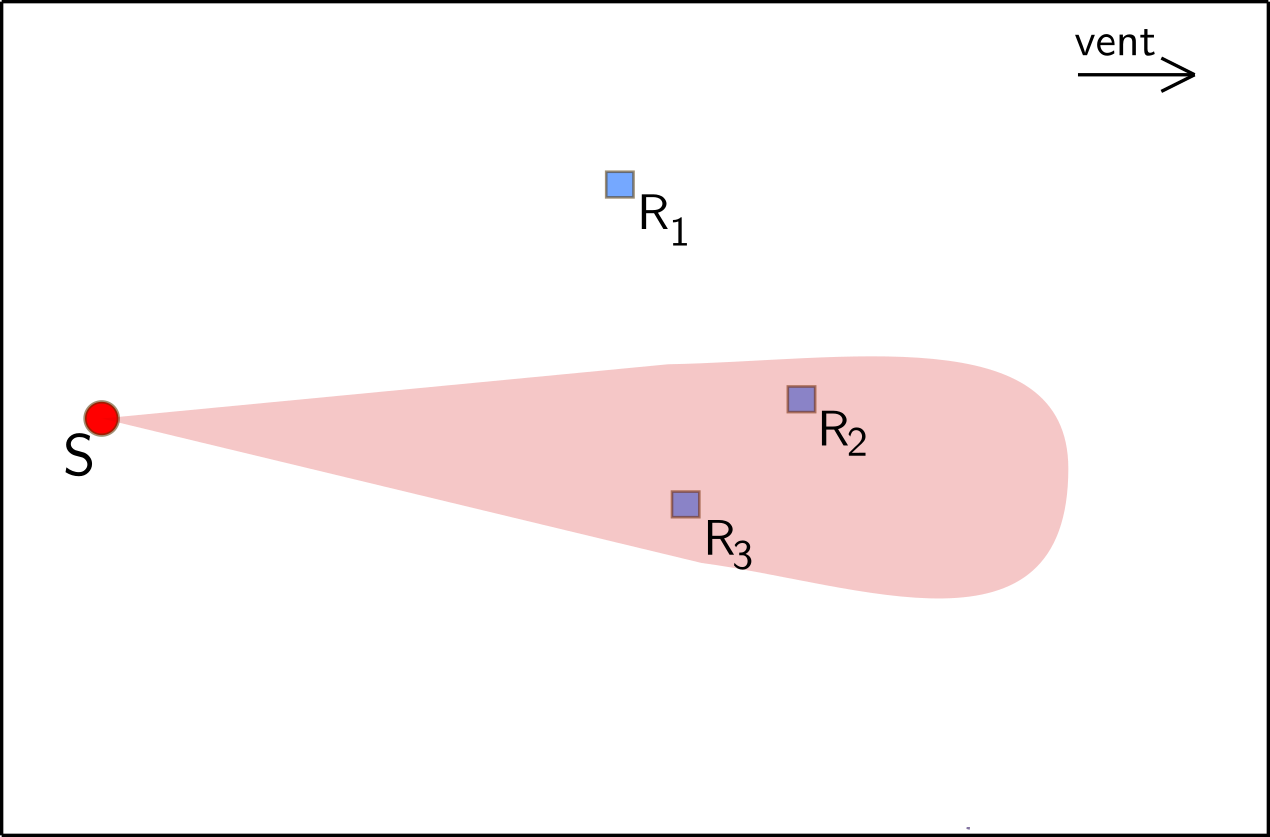
\includegraphics[scale=0.6]{schema_probleme_direct.png}
			\caption{Approche orientée source}
			\label{schema_probleme_direct}
		\end{subfigure}
		\begin{subfigure}{0.5\textwidth}
		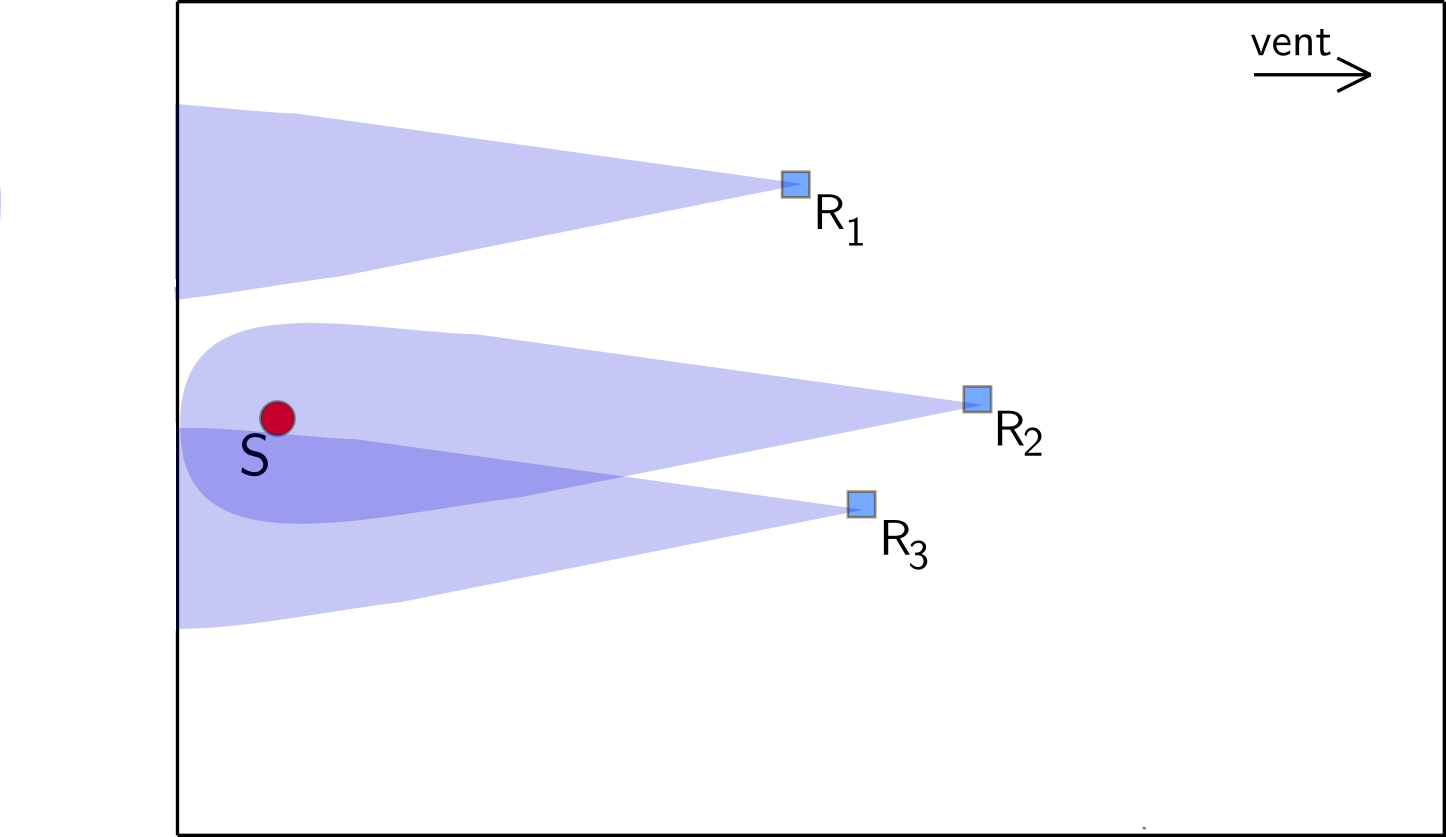
\includegraphics[scale=0.2]{schema_probleme_inverse.png}
		\caption{Approche orientée récepteur}
		\label{schema_probleme_inverse}
	\end{subfigure}
	\caption{Exemple illustrant la relation entre une source unique $S$ et trois capteurs $R_1,R_2,R_3$ sur un problème en deux dimensions pour une approche directe (\ref{schema_probleme_direct}) et une approche adjointe (\ref{schema_probleme_inverse}). }
	\end{figure}
	

	La solution $C^*$ de l'équation \eqref{eqn_advection_diffusion_backward} permet ainsi de reconstruire un champ d'émission et de caractériser la source recherchée. Cette méthode est appliquée dans \cite{Pudykiewicz1998}, où la position et l'intensité du terme source de Tchernobyl sont reconstruits. De même, dans \cite{Hourdin2006b} le principe du \textit{backtracking} est appliqué à un modèle eulérien pour retrouver la source de la campagne ETEX\footnote{L’expérience \textit{European Tracer EXperiment} (ETEX), menée en 1997,  a consisté à mesurer et étudier l'impact à l'échelle européenne de rejets de gaz traceurs passifs émis depuis le nord de la France \cite{Nodop1998}.}.
	
	 Dans \cite{Robertson1998}, l'inversion est faite dans le cadre de l'assimilation de données: cette méthodologie permet de corriger de façon variationnelle les paramètres du modèle de dispersion selon une boucle de rétro-action basée sur des observations. Très utilisée en météorologie, l'assimilation de données agit en deux temps selon un principe de "prévision-correction", et itère sur le cycle suivant:
	\begin{enumerate}
		\item  on calcule d'abord une ébauche de l'état à l'instant présent $t$, en appliquant un modèle de prévision en $t-1$,
		\item  on exploite ensuite les observations disponibles à l'instant $t$ pour corriger les paramètres du modèle en les comparant avec l'ébauche. \\
	\end{enumerate}
	
	\cite{Issartel2005} mentionne le principe d'\textit{illumination}, qui est une mesure quantitative de la représentativité des mesures dans le temps et l'espace. Dans le cadre d'un modèle adjoint, l'illumination permet ainsi de caractériser des zones qui ne sont pas forcément couvertes par les rétro-émissions issues des capteurs, par exemple si la zone considérée est relativement éloignée du point de mesure le plus proche. Cependant, si l'information d'illumination est utilisée pour inverser un terme source, alors elle aura tendance à fortement favoriser les solutions proches des capteurs. Pour compenser ce problème, une phase de \textit{renormalisation} est introduite (\cite{Issartel2007} et \cite{Sharan2009}) pour équilibrer l'information apportée par chacun des capteurs. D'abord utilisée à grande échelle, cette méthodologie a récemment été validée à l'échelle locale dans \cite{Singh2014}, et dans un contexte urbain par \cite{Kumar2015}.
	
	
	
	


 \subsection{Méthodes évolutionnaires}
 
 Les \textit{approches évolutionnaires}, dont les \textit{algorithmes génétiques} font partie, sont des méthodes d'optimisation s'inspirant de l'évolution darwinienne des populations biologiques. La conception de ces algorithmes s'appuie sur le fait que l'apparition d'espèces adaptées au milieu est la conséquence de la conjonction de deux phénomènes distincts : 
 \begin{itemize}
 	\item d'une part, la \textit{sélection naturelle} imposée par le milieu (les individus les plus adaptés survivent et se reproduisent),
 	\item d'autre part, les variations non-contrôlées du matériel génétique des espèces.
 \end{itemize}
 
 Pour un problème d'optimisation standard, la fonction-coût $\CostF$ à minimiser devient, dans le langage évolutionnaire, une \textit{fonction d'adaptation}. Les points du domaine $\Omega$ des paramètres à explorer sont appelés \textit{individus}, et l'ensemble d'individus est appelé \textit{population}. \\
 
 La structure d'un algorithme évolutionnaire se compose de plusieurs étapes. Dans un premier temps, on initialise une population $\Pi_0$ en tirant $p$ individus dans $\Omega$ de façon uniformément aléatoire, et on l'évalue en calculant les valeurs de $\CostF$ pour chaque individu. Vient ensuite une boucle itérative qui implémente le processus de sélection naturelle:
 \begin{enumerate}
 	\item on sélectionne les individus les plus performants (au sens de $\CostF$) de la population $\Pi_i$ à l'itération courante $i$, que l'on appelle \textit{parents},
 	\item on applique des opérateurs de variation aux parents sélectionnés, pour générer de nouveaux individus: les \textit{enfants}. On parle de mutation si l'opérateur est 1-aire (i.e. ne prend qu'un seul individu en argument) et de croisement si l'opérateur est $n$-aire (i.e. prend $n$ individus en argument, avec $n \geq 2$). Notons que cette étape est purement stochastique, et que les opérateurs n'utilisent pas d'information sur la performance des précédentes générations: on parle alors d'opérateurs semi-aveugles.
 	\item on évalue les enfants avec $\CostF$,
 	\item on remplace $\Pi_i$  par une nouvelle population $\Pi_{i+1}$ créée à partir des enfants et des parents de $\Pi_i$ au moyen d'une sélection darwinienne.\\
 \end{enumerate}
 
 Dans notre contexte, on peut assimiler $\Omega$ à l'espace des paramètres du terme source. Historiquement, les premières méthodes d'estimation basées sur les algorithmes génétiques (voir par exemple \cite{Haupt2005}) supposaient connues certaines informations a priori comme les emplacements potentiels de la source. Dans \cite{Allen2007} et \cite{Haupt2007}, il est envisagé de se placer dans une situation plus réaliste où les paramètres à estimer comprennent non seulement la position de la source et la masse totale émise, mais également la vitesse et la direction du vent. \cite{Cervone2011} propose une extension du processus de variation en couplant les opérateurs de croisement et de mutation avec un algorithme non-darwinien d'inférence statistique.\\ 
 
 Une telle approche a également permis d'étudier le rapport entre la précision du terme source reconstruit et le nombre de capteurs utilisés. \cite{Long2010} reprend ce problème de précision en testant un algorithme génétique sur différentes configurations de réseaux de capteurs plus ou moins denses, et en prenant en compte le caractère bruité des données fournies par les détecteurs. \\
 
 L'approche génétique a récemment été validée sur des données expérimentales de rejet multi-sources, comme présenté dans les travaux de \cite{Cantelli2015} où jusqu'à trois sources distinctes ont pu être caractérisées.\\
 
 \subsection{Méthodes bayésiennes déterministes}
 
 Si on reprend la notation de l'équation \eqref{eq_relation_SR_non_parametrique}, une vision \textit{bayésienne} du problème consiste à estimer la probabilité a posteriori $p(\VecSigma | \VecObs)$ après obtention des observations $\VecObs$. Il s'agit pour cela de combiner de l'information a priori (obtenue grâce à un ensemble d'hypothèses de départ) et l'ajout d'information nouvelle en utilisant à la fois les observations et un modèle de dispersion. Cela peut être fait grâce à la \textit{règle de Bayes}, qui s'exprime sous la forme suivante: 
 
 \begin{equation}
	 \label{eq_regle_bayes_deterministe}
	 p(\VecSigma | \VecObs) = \dfrac{p(\VecSigma)p(\VecObs | \VecSigma)}{p(\VecObs)}
 \end{equation}
 où:
 \begin{itemize}
 	\item $p(\VecObs | \VecSigma)$ est la densité de probabilité des mesures $\VecObs$ étant donnée une source $\VecSigma$, aussi appelée \textit{loi de vraisemblance},
 	\item $p(\VecSigma)$ est la densité de probabilité de la source $\VecSigma$ avant obtention des mesures $\VecObs$, aussi appelée \textit{loi a priori},
 	\item $p(\VecObs)$ est la vraisemblance marginale des mesures.\\
 \end{itemize}
 
 Pour obtenir un estimateur fiable de $\VecSigma$, une méthode habituellement utilisée est celle de la maximisation de la probabilité a posteriori: 
 
 \begin{equation}
	 \label{eq_maximum_posterior}
	 \hat{\VecSigma} = \argmax_\sigma \left(p(\VecSigma | \VecObs)\right)
 \end{equation}
 
 Pour construire cet estimateur, il est nécessaire de caractériser les statistiques des erreurs d'observation $\VecErreur$. Pour cela on peut définir sa matrice de covariance $\bm{R} \in \mathbb{R}^{m\times m}$ par: 
 
 \begin{equation}
	 \label{eq_matrice_R}
	 \MatR = \mathbb{E}[\VecErreur \VecErreur^T]
 \end{equation}
 
 On peut également définir une \textit{ébauche} (ou \textit{first-guess}) $\VecSigma_b$ de la source recherchée : l'erreur d'ébauche $\VecSigma - \VecSigmaB$ est alors caractérisée par la matrice de covariance $\MatB \in \mathbb{R}^{N_\sigma \times N_\sigma}$ définie par:\\
 
 
 \begin{equation}
	 \label{eq_matrice_B}
	 \MatB = \mathbb{E}[(\VecSigma - \VecSigmaB)(\VecSigma - \VecSigmaB)^T]
 \end{equation}
 
 Si on suppose que les erreurs d'observation et d'ébauche : \\
 
 \begin{itemize}
 	\item sont non-biaisées: $\mathbb{E}[\VecErreur] = 0$ et $\mathbb{E}[\VecSigma - \VecSigmaB] = 0$,
 	\item suivent une loi normale: $\VecErreur \sim  \mathcal{N}(0,\MatR)$ et $\VecSigma - \VecSigmaB \sim \mathcal{N}(0,\MatB)$,\\
 \end{itemize}
 
 alors maximiser la probabilité a posteriori revient à minimiser la fonction-coût suivante \cite{Winiarek2011}:
 
 \begin{equation}
	 \label{eq_fonction_cout_3dvar}
	 \CostF(\VecSigma) = \dfrac{1}{2}(\VecObs - \MatH\VecSigma)^T \MatR^{-1} (\VecObs - \MatH\VecSigma) + \dfrac{1}{2}(\VecSigma - \VecSigmaB)^T \MatB^{-1}(\VecSigma - \VecSigmaB)
 \end{equation}
 
 On a donc, dans ce cas, équivalence entre une formulation bayésienne et une méthode des moindres carrés telle que présentée dans \cite{Davoine2007}, où le deuxième terme de la somme dans l'équation \eqref{eq_fonction_cout_3dvar} peut être vu comme l'analogue du terme régularisant de Tikhonov \cite{Tikhonov1963}.\\
 
 L'obtention du terme source recherché dans \eqref{eq_maximum_posterior} peut alors se faire en résolvant le problème suivant:
 
 \begin{equation}
	 \label{eq_argmin_3dvar}
	 \hat{\VecSigma} = \argmin_\sigma (\CostF)
 \end{equation}
 
 grâce à des méthodes à base de descente de gradient, en calculant  par exemple le \textit{Best Linear Unbiased Estimator}, ou estimateur BLUE, comme présenté dans \cite{Winiarek2012}. \\
 
 Dans le même cadre, \cite{Saunier2013} propose une reconstruction du terme source de l'accident de Fukushima en deux temps. Tout d'abord, une première fonction-coût est minimisée pour estimer la période du rejet, puis tenant compte de cette contrainte, une seconde fonction-coût est optimisée pour retrouver la source à proprement parler. 
 Il est à noter que l'équation \eqref{eq_fonction_cout_3dvar} correspond à celle de la méthode d'assimilation variationnelle de données 3D-var \cite{Courtier1998}. La vision de ce type d'estimation se rapproche ainsi de celle de l'assimilation de mesures issues de capteurs pour reconstruire un état inconnu, qui est ici le champ d'émission de la source recherchée.\\
 
 Une variante pour cette approche consiste à se placer dans un cadre statistique non-gaussien, notamment si on cherche à caractériser l'ébauche suivant certaines hypothèses spécifiques \cite{Bocquet2005a}. Les auteurs de \cite{Krysta2007} font l'hypothèse d'une source ponctuelle et instantanée pour définir une forme particulière d'ébauche, et utilisent un principe de maximum d'entropie sur la moyenne \cite{Jaynes1957} pour réécrire la fonction-coût et en dériver un estimateur approprié pour $\VecSigma$.\\
  

 \subsection{Méthodes bayésiennes stochastiques}
 
 Dans les cas où le nombre d'observations est limité, et la position de la source est inconnue (par exemple, dans un contexte accidentel), la dimension $N_\sigma$ du vecteur d'état $\VecSigma$ à estimer est supérieure à $m$, qui est celle du vecteur d'observation $\VecObs$. Le problème est alors qualifié de "mal-posé". Dans certaines méthodes évoquées précédemment, il était possible de "régulariser" le problème d'un point de vue physique en introduisant un terme d'ébauche. \\
 
 Une autre logique consiste à formuler une hypothèse forte sur la source en la supposant réduite spatialement à un point de l'espace, ce qui revient à écrire l'équation \eqref{eq_relation_SR_parametrique} et \textit{de facto} régulariser le problème, car le nombre de paramètres contenus dans $\VecTheta$ devient alors largement inférieur à $N_\sigma$ et à $m$. On passe en effet de $N_xN_yN_z$ paramètres spatiaux à 3 composantes $(x_s, y_s, z_s)$ dans le cas d'une source unique. Il est ainsi possible de combiner cette formulation avec une approche bayésienne pour chercher à calculer la probabilité a posteriori $p(\VecTheta | \VecObs)$. \\
 
 On peut prendre comme premier exemple l'étude menée par \cite{Sohn2002}, qui se penche sur le cas particulier de l'estimation de source à l'intérieur d'un bâtiment. Pour cela, un premier calcul simule un nombre $N$ fixé de scénarios $S_1,\dots,S_N$ possibles à partir d'un échantillon de paramètres $\VecTheta_1, \dots, \VecTheta_N$ potentiels de la source. Chaque scénario $S_k$ représente un jeu de mesures simulées issues d'une source de paramètres $\VecTheta_k$. Une fois cette collection constituée, la loi a posteriori suivante est calculée via la règle de Bayes, pour chaque scénario $S_k$:
 
 \begin{equation}
	 \label{eq_bayes_monte_carlo}
	 p(S_k|\VecObs) = \dfrac{p(S_k)p(\VecObs | S_k)}{p(\VecObs)}
 \end{equation}
 
 Cette première approche, appelée \textit{Bayes Monte Carlo} (BMC), permet de caractériser un rejet mais peut également servir à placer de façon optimale les capteurs d'un réseau de mesure. \\
 
 Toutefois, l'expression analytique d'une loi a posteriori n'est généralement  pas accessible de façon directe, du fait de la forte non-linéarité des phénomènes pris en compte par le modèle de dispersion. Il est alors nécessaire d'introduire des méthodes numériques d'approximation pour évaluer  $p(\VecTheta | \VecObs)$. En général, il s'agit d'algorithmes de simulation aléatoire appartenant à la famille des méthodes de Monte-Carlo, et qui permettent une exploration optimale de l'espace des solutions.\\
 
 Parmi ces algorithmes, la catégorie la plus connue est certainement celle des méthodes dites \textit{Markov Chain Monte-Carlo} (MCMC). Dans \cite{Chow2008}, la méthode MCMC est employée dans un contexte urbain, et couplée à un modèle de type CFD pour tenir compte de la géométrie complexe de l'environnement. \cite{Senocak2008} propose un modèle plus simple de type gaussien, amélioré par l'ajout de paramètres stochastiques relatifs à la diffusion turbulente, eux-mêmes estimés par l'algorithme MCMC en plus des paramètres de la source. \\
 
 Les exemples précédemment cités couplent un algorithme bayésien avec un modèle de dispersion direct. Il est néanmoins possible d'adopter une approche orientée récepteur, comme présenté dans \cite{Keats2007}, ce qui permet une exploitation plus efficace des calculs de dispersion. \cite{Yee2008b} étend cette métholodogie aux cas où le nombre de sources est inconnu et considéré comme un paramètre supplémentaire à estimer. Cela est possible grâce à une méthode MCMC à \textit{sauts réversibles}, qui associe pour chaque nombre de sources possible un espace de paramètres différent à explorer. Enfin, \cite{Yee2014} propose une extension des concepts de \cite{Keats2007} à l'échelle globale, où un algorithme MCMC est utilisé pour reconstruire la position et le profil d'émission d'une usine d'isotopes médicaux à partir des mesures de xénon-133 relevés par le réseau mondial des capteurs de l'OTICE\footnote{L'\textit{Organisation du Traité d'Interdiction Complète des Essais Nucléaires} (OTICE, ou CTBTO en anglais: \textit{Comprehensive Nuclear-Test Ban Treaty Organization)} a pour rôle de détecter, grâce à un réseau de capteurs déployés sur l'ensemble du globe, et de signaler à tous les pays signataires du traité toute explosion d'origine atomique, pour prendre des mesures afin d'empêcher les puissances nucléaires actuelles de poursuivre leurs essais, et les Etats ne disposant pas de l'arme atomique de s'en doter.}. \\
 
 %\todo[inline]{Dans le cadre de ce manuscrit, la méthodologie MCMC est expliquée avec plus de détails au Chapitre 2 pour les aspects théoriques, et un exemple pratique d'application est illustré au Chapitre 3.\\}
 
 \section{Problématique de recherche}
 
 Le développement des méthodes STE dans le contexte de la dispersion atmosphérique est une branche scientifique relativement récente par rapport au cadre général de la physique de l'atmosphère. Il s'agit également d'un domaine de recherche largement pluridisciplinaire, mêlant des compétences en physique mais également sur des aspects mathématiques (optimisation, statistiques, simulation aléatoire...) et informatique (algorithmique, calcul scientifique haute performance...) variés. \\
 
 Même si de nombreux aspects sont couverts par les éléments présents dans l'état de l'art exposé en paragraphe §\ref{section_etat_art_STE}, de nombreuses questions restent encore ouvertes. Dans le cas particulier de situations accidentelles, il est ainsi important pour les primo-intervenants de disposer d'une information fiable avec une certaine quantification de l'incertitude, à partir d'un nombre potentiellement faible de mesures, et dans un intervalle de temps raisonnablement court pour assurer l'efficacité de l'intervention. Les questions de vitesse de calcul sont alors, de fait, importantes: si elles ne posent pas de problèmes dans le cadre d'une étude \textit{a posteriori}, il en va autrement en situation de crise, où le temps de réponse à un incident est un paramètre primordial. Un autre aspect majeur est celui de la nature de la source à retrouver. Pour le contexte accidentel, si on se place dans le cas d'un attentat à la bombe sale ou dans celui d'une fuite sur un complexe industriel, l'hypothèse d'une source localisée est raisonnable. Toutefois il peut être intéressant de se pencher plus en détail sur le profil du rejet, celui-ci n'étant pas forcément instantané, alors que plusieurs méthodes privilégient l'estimation d'un unique instant d'émission $t'_s$. \\
 

\textit{Les travaux présentés dans ce manuscrit et ayant fait l'objet du travail de thèse ont donc pour but: }
 	
 	\begin{itemize}
 		\item \textit{de développer et valider une méthode basée sur l'inférence bayésienne, capable de caractériser un point source par sa localisation et son profil de rejet à partir de mesures issues d'un réseau de capteurs, }
 		\item \textit{de coupler cette méthode avec un modèle de dispersion atmosphérique développé par ARIA Technologies et le CEA au sein d'une chaîne de calcul pouvant, à terme, être utilisée en situation opérationnelle.} \\
 	\end{itemize}

 
 Pour cela, nous avons recours à une approche de type Monte-Carlo différente des MCMC de par sa philosophie, et basée sur un principe d'échantillonnage d'importance adaptatif. De telles méthodes permettent en effet une convergence suffisamment rapide, et pallient certaines difficultés rencontrées par les MCMC. Nous associons cette méthode adaptative, utilisée pour localiser la source, à un calcul analytique du profil d'émission, permis par le choix d'une hypothèse de gaussianité sur le vecteur $\VecSigma$, et accompagné par l'implémentation d'une étape de contrainte visant à assurer la positivité de $\VecSigma$. Le schéma d'implémentation que nous avons conçu permet ainsi de produire une estimation des paramètres de position et d'émission d'une source unique via un schéma itératif de couplage avec un modèle de dispersion, la procédure d'estimation à proprement parler demeurant indépendante du modèle choisi. \\
 
 Pour développer cette thèse, le présent manuscrit est organisé de la façon suivante. Après avoir présenté la problématique posée par le sujet et effectué un premier tour d'horizon de la thématique dans ce chapitre introductif, nous développons au Chapitre 2 les principes régissant l'inférence bayésienne, en nous concentrant plus particulièrement sur les applications des méthodes de Monte-Carlo en statistique bayésienne. Nous y détaillons notamment le cheminement théorique permettant la construction de l'algorithme AMIS, qui constitue un élément central des travaux de cette thèse. 
 Dans le Chapitre 3, nous présentons l'application de cet algorithme adaptatif à la question de la reconstruction du terme source en dispersion atmosphérique. Pour cela, nous exploitons un cas d'application pratique issu d'une campagne de mesures expérimentales dont nous expliquerons les conditions de réalisation. Le Chapitre 4 détaille une variante de la méthodologie présentée au Chapitre 3, avec l'utilisation d'une approche orientée récepteur, et l'emploi d'un code de dispersion de type lagrangien dans des configurations simulées de rase campagne et de milieu urbain.
 Enfin, le Chapitre 5 conclut ce manuscrit et discute de plusieurs perspectives pour de futurs axes de prolongement de ces travaux.\\